\documentclass[11pt]{standalone}
\usepackage{physics}			% Vector stuff
\usepackage{tikz}
\usetikzlibrary{angles, calc, decorations.pathmorphing, quotes, spy}

\begin{document}
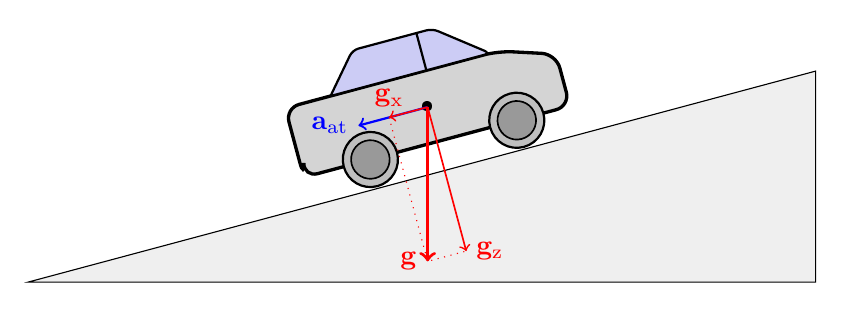
\begin{tikzpicture}[scale=1]
    % Define/Calc ramp parameters
    % Ramp length
    \def\rl{10};
    % Ramp angle [deg]
    \def\ra{15};
    % Ramp height
    \def\rh{{tan(\ra)*\rl}};

    % RAMP
    % Define the points
    \coordinate (A) at (0,0);
    \coordinate (B) at ($(A) + (\rl,0)$);
    \coordinate (C) at ($(B) + (0,\rh)$);
    % Draw and fill ramp
    \filldraw[draw=black, fill=lightgray!25] (A) -- (B) -- (C) -- cycle;

    % CAR
    % Tilt whole car
    \begin{scope}[scale=0.7, xshift=\rl*0.5 cm, yshift=1.9 cm, rotate=\ra]
        % Car height
        \def\ch{2}
        % Car length
        \def\cl{5}
        % Car body height
        \def\bh{\ch*0.65}
        % Roof length
        \def\rl{\cl*0.6}
        % Roof height
        \def\rh{\ch*0.35}
        % Car tilt angle
        \def\ct{6}

        % Anchor point is southwest
        \coordinate (b) at (0,0);
        % Offset to roof and wheels
        \coordinate (r) at ($(b) +(\cl*0.17,\ch*0.65)$);
        \coordinate (w) at ($(b) + (\cl*0.25,0)$);
        % Body
        \draw[black, fill=black!17, rounded corners=1.2ex, very thick]
        (b) -- ++(0,\bh) -- ++(\cl*1/5,0) --  ++(\cl*3/5,0) -- ++(\cl*1/5,-\bh*0.25)
        -- ++(0, -\bh*0.75) -- (b) -- cycle;
        % Roof
        \draw[very thick, rounded corners=0.5ex, fill=black!20!blue!20!white,thick]
        (r) -- ++(0.2*\rl,\rh) -- ++(0.5*\rl,0) -- ++(0.3*\rl,-\rh) -- (r);
        \draw[thick] (r)++(\rl*0.6,0) -- ++(0,\rh);

        % % Car middle point
        \coordinate (m) at (\cl*0.5, \bh*0.5);
        \node at (m) {\textbullet};
        % Wheels
        \draw[draw=black,fill=gray!50,thick] (w) circle (.5);
        \draw[draw=black,fill=gray!50,thick] (w) ++(\cl*0.55,0) circle (.5);
        % Inner wheels
        \draw[draw=black,fill=gray!80,semithick] (w) circle (.35);
        \draw[draw=black,fill=gray!80,semithick] (w) ++(\cl*0.55,0) circle (.35);

        % Draw car acceleration
        \draw[blue, thick, ->] (m) -- ++(-1.3,0) node[anchor=east]{$\vb{a}_\mathrm{at}$};
        % Gravity vectors
        % Length of g vector
        \def\gl{2.8}
        % Length of g vector components
        \def\gxl{{\gl*sin(\ra)}}
        \def\gzl{{\gl*cos(\ra)}}
        % Draw vectors
        \draw[red, ->, very thick, rotate=-\ra] (m) -- ++(0,-\gl) node[anchor=east](g_end){$\vb{g}$};
        \draw[red, semithick, ->] (m) -- ++(-\gxl,0) node[anchor=south]{$\vb{g}_\mathrm{x}$};
        \draw[red, semithick, ->] (m) -- ++(0,-\gzl) node[anchor=west]{$\vb{g}_\mathrm{z}$};
        \draw[red, dotted] ($(m)+(-\gxl,0)$) -- ++(0,-\gzl) -- ++(\gxl,0);
        % \draw[red, dotted] ($(m)+(0,0)$) -- ++(0,-\gzl) -- ++(\gxl,0);
    \end{scope}
\end{tikzpicture}
\end{document}